% ============================================================
% ECON 308 — International Economic Relations
% Lecture 1: World Trade — An Overview (Chapter 2)
% Fall 2026  |  Muhebullah Karimzada  |  UNBC
% ============================================================
\documentclass[aspectratio=169]{beamer}
\usepackage[utf8]{inputenc}
\usepackage[T1]{fontenc}
\usepackage{lmodern}

%% ── Theme and colours ───────────────────────────────────────
\usetheme{Madrid}
\setbeamertemplate{navigation symbols}{}
\setbeamercovered{transparent}
\setbeamertemplate{itemize items}[circle]
\setbeamertemplate{enumerate items}[default]
\setlength{\parskip}{0.2em}

\definecolor{UNBCDark}  {RGB}{0,74,37}
\definecolor{UNBCGold}  {RGB}{189,155,96}
\definecolor{SoftGray}  {RGB}{244,246,248}
\definecolor{AccentRed} {RGB}{192,57,43}
\definecolor{AccentBlue}{RGB}{41,98,255}
\definecolor{AccentTeal}{RGB}{0,150,136}
\definecolor{AccentOrange}{RGB}{230,126,34}

\setbeamercolor{normal text}       {fg=black,bg=white}
\setbeamercolor{structure}         {fg=UNBCDark}
\setbeamercolor{title}             {fg=white,bg=UNBCDark}
\setbeamercolor{subtitle}          {fg=UNBCGold}
\setbeamercolor{frametitle}        {fg=white,bg=UNBCDark}
\setbeamercolor{block title}       {fg=white,bg=UNBCDark}
\setbeamercolor{block body}        {fg=black,bg=SoftGray}
\setbeamercolor{block title alerted}{fg=white,bg=AccentRed}
\setbeamercolor{block body alerted}{fg=black,bg=SoftGray}
\setbeamercolor{item}              {fg=UNBCDark}
\setbeamercolor{alerted text}      {fg=AccentRed}
\setbeamercolor{author in head/foot}{fg=white,bg=UNBCDark}
\setbeamercolor{date in head/foot} {fg=white,bg=UNBCDark}

%% ── Packages ────────────────────────────────────────────────
\usepackage{booktabs,multirow,array,amsmath,amssymb,bm,graphicx,adjustbox}
\usepackage{tikz,pgfplots,multicol,tcolorbox,hyperref}
\tcbuselibrary{skins}
\pgfplotsset{compat=1.18}
\usetikzlibrary{arrows.meta,positioning,calc,decorations.pathreplacing,shapes.geometric}
\hypersetup{colorlinks=true,linkcolor=UNBCDark}

%% ── Footline ────────────────────────────────────────────────
\setbeamertemplate{headline}{}
\setbeamertemplate{footline}{%
  \leavevmode\hbox{%
  \begin{beamercolorbox}[wd=.78\paperwidth,ht=2.8ex,dp=1.2ex,leftskip=1em]{author in head/foot}%
    \color{white}\textbf{ECON 308}\hspace{0.4em}%
    \textcolor{UNBCGold}{$\vert$}\hspace{0.4em}International Economic Relations%
  \end{beamercolorbox}%
  \begin{beamercolorbox}[wd=.22\paperwidth,ht=2.8ex,dp=1.2ex,rightskip=1em plus 1fil]{date in head/foot}%
    \color{white}\hfill\insertframenumber/\inserttotalframenumber%
  \end{beamercolorbox}}%
}

%% ── Custom boxes ────────────────────────────────────────────
\newtcolorbox{insight}[1]{
  colback=UNBCGold!12,colframe=UNBCGold!70!black,
  title={\small\bfseries #1},
  left=1.5mm,right=1.5mm,top=0.6mm,bottom=0.6mm,
  boxrule=0.5pt,arc=2mm}

\newtcolorbox{canadex}[1][Canadian Example]{
  colback=AccentTeal!9,colframe=AccentTeal,
  title={\small\bfseries #1},
  left=1.5mm,right=1.5mm,top=0.6mm,bottom=0.6mm,
  boxrule=0.5pt,arc=2mm}

\newtcolorbox{discuss}{
  colback=AccentBlue!8,colframe=AccentBlue,
  title={\small\bfseries Discussion},
  left=1.5mm,right=1.5mm,top=0.6mm,bottom=0.6mm,
  boxrule=0.5pt,arc=2mm}

\newtcolorbox{worked}{
  colback=AccentOrange!8,colframe=AccentOrange,
  title={\small\bfseries Worked Example},
  left=1.5mm,right=1.5mm,top=0.6mm,bottom=0.6mm,
  boxrule=0.5pt,arc=2mm}

\newtcolorbox{varbox}{
  colback=SoftGray,colframe=UNBCDark!45,
  left=1.5mm,right=1.5mm,top=0.6mm,bottom=0.6mm,
  boxrule=0.4pt,arc=2mm}

%% ── Figure helpers ──────────────────────────────────────────
% Full-column figure (use inside a column)
\newcommand{\FIG}[1]{%
  \begin{center}%
  \includegraphics[width=\columnwidth,height=0.63\textheight,keepaspectratio]{#1}%
  \end{center}}

% Scaled figure
\newcommand{\FIGS}[2][0.90]{%
  \begin{center}%
  \includegraphics[width=#1\columnwidth,height=0.63\textheight,keepaspectratio]{#2}%
  \end{center}}

%% ── Metadata ────────────────────────────────────────────────
\title{\textbf{World Trade: An Overview}}
\subtitle{{\large ECON 308 \enspace International Economic Relations
           \enspace\textcolor{UNBCGold}{$|$}\enspace Chapter~2}}
\author{Muhebullah Karimzada}
\institute{School of Economics\\University of Northern British Columbia}
\date{Fall 2026}

% ============================================================
\begin{document}
% ============================================================

%% ─────────────────────────────────────────────────────────────
%% TITLE
%% ─────────────────────────────────────────────────────────────
\begin{frame}[plain]
\titlepage
\end{frame}

%% ─────────────────────────────────────────────────────────────
%% 1. WHY THIS MATTERS FOR CANADA
%% ─────────────────────────────────────────────────────────────
\begin{frame}{Why Trade Matters: Canada's Economy Depends on It}
\begin{columns}[T]
\begin{column}{0.54\textwidth}
\begin{itemize}
  \item Canada is among the world's \textbf{most trade-dependent} advanced economies.
  \item \textbf{Exports $\approx$ 32\% of GDP}; imports $\approx$ 33\% (2023).
  \item A 10\% drop in Canadian exports is a \textbf{$\approx$3\% shock to nominal GDP} - larger than most recessions.
  \item Trade drives jobs, wages, prices, and the business cycle.
\end{itemize}
\vspace{0.3em}
\begin{canadex}[Canada's Top Exports, 2023]
\footnotesize
Crude oil \$136B $\cdot$ Cars/parts \$65B $\cdot$ Gold \$22B $\cdot$ Natural gas \$17B $\cdot$ Lumber \$14B.
\textbf{75\% of all Canadian exports go to the United States.}
\end{canadex}
\end{column}
\begin{column}{0.43\textwidth}
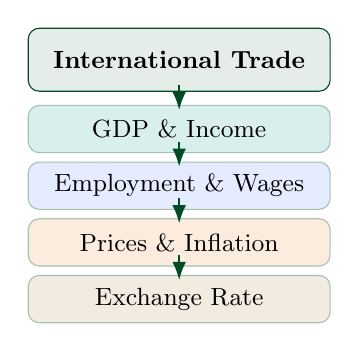
\begin{tikzpicture}[scale=0.80,every node/.style={font=\small}]
  \node[draw=UNBCDark,fill=UNBCDark!10,rounded corners,
        text width=3.6cm,minimum height=0.8cm,align=center,
        font=\small\bfseries] (T) at (0,4.0)
    {International Trade};
  \foreach \y/\fc/\t in {
      2.9/AccentTeal!15/{GDP \& Income},
      2.0/AccentBlue!12/{Employment \& Wages},
      1.1/AccentOrange!15/{Prices \& Inflation},
      0.2/UNBCGold!20/{Exchange Rate}}{
    \node[draw=UNBCDark!35,fill=\fc,rounded corners,
          text width=3.6cm,minimum height=0.6cm,align=center,
          font=\small]
      at (0,\y) {\t};
  }
  \foreach \ya/\yb in {3.6/3.2,2.7/2.3,1.8/1.4,0.9/0.5}
    \draw[-{Latex},UNBCDark,thick] (0,\ya)--(0,\yb);
\end{tikzpicture}
\end{column}
\end{columns}
\end{frame}

%% ─────────────────────────────────────────────────────────────
%% 2. TRADE–MACRO NEXUS
%% ─────────────────────────────────────────────────────────────
\begin{frame}{The Trade–Macro Nexus: GDP and Net Exports}
\begin{columns}[T]
\begin{column}{0.55\textwidth}
\textbf{In the expenditure approach to GDP:}
\vspace{0.2em}
\[Y \;=\; C + I + G + \underbrace{(X - M)}_{\text{Net exports (NX)}}\]
\begin{varbox}
\footnotesize
$Y$ = real GDP \hfill $C$ = household consumption\\
$I$ = business investment \hfill $G$ = government spending\\
$X$ = exports \hfill $M$ = imports\\[0.2em]
$\text{NX} = X - M$ \;=\; \textbf{trade balance}\\
NX $>0$: trade surplus (\,Canada exports more than it imports\,)\\
NX $<0$: trade deficit
\end{varbox}
\vspace{0.3em}
\textbf{Key insight:} When exports fall (e.g.\ US recession), NX falls, and so does $Y$ -- directly contracting the Canadian economy.
\end{column}
\begin{column}{0.42\textwidth}
\begin{insight}{Canada's (X$-$M)/GDP}
\footnotesize
\begin{adjustbox}{max width=\columnwidth}
\begin{tabular}{lcc}
\toprule
Year & $X/Y$ & $(X-M)/Y$\\
\midrule
2000 & 45\% & $+$5.0\%\\
2008 & 33\% & $+$0.5\%\\
2015 & 32\% & $-$3.2\%\\
2022 & 32\% & $+$1.1\%\\
\bottomrule
\end{tabular}
\vspace{0.3em}
\end{adjustbox}\\

Canada's trade balance swings between surplus and deficit with commodity prices and US demand - both \emph{international} forces with large \emph{domestic} consequences.
\end{insight}
\end{column}
\end{columns}
\end{frame}

%% ─────────────────────────────────────────────────────────────
%% 3. LEARNING OBJECTIVES
%% ─────────────────────────────────────────────────────────────
\begin{frame}{Learning Objectives}
After this lecture you will be able to:
\begin{enumerate}
  \item Describe why large, nearby economies trade the most with each other.
  \item State and interpret the \textbf{gravity model} at three levels: intuition, equation, and general equilibrium.
  \item Solve a \textbf{numerical gravity problem} and interpret the coefficients.
  \item Explain why national \textbf{borders} and \textbf{distance} substantially deter trade even in the digital era.
  \item Trace the \textbf{two waves of globalisation} and the forces that reversed each.
  \item Characterise how the \textbf{composition} of world trade has evolved since 1945.
  \item Explain how a trade shock transmits to \textbf{Canadian macro outcomes} (GDP, employment, monetary policy).
\end{enumerate}
\begin{block}{Reference}
  Krugman, Obstfeld \& Melitz, \textit{International Economics: Theory and Policy}, 12th ed., Chapter~2.
\end{block}
\end{frame}

%% ═══════════════════════════════════════════════════════════
%%  PART 1 — FACTS OF WORLD TRADE
%% ═══════════════════════════════════════════════════════════

%% ─────────────────────────────────────────────────────────────
%% 4. WHO TRADES WITH WHOM
%% ─────────────────────────────────────────────────────────────
\begin{frame}[shrink=6]{Who Trades with Whom? The Basic Facts}
\begin{columns}[T]
\begin{column}{0.55\textwidth}
\begin{itemize}
  \item More than \textbf{30\% of world output} crosses national borders every year.
  \item World merchandise trade exceeded \textbf{\$25 trillion in 2019}.
  \item Trade is \textbf{highly concentrated}: the top-15 US partners account for \textbf{75\%} of all US trade.
  \item Top-5 US partners (2019): \textbf{Mexico, Canada, China, Japan, Germany}.
  \item The pattern: \textbf{large} economies and \textbf{nearby} economies dominate.
\end{itemize}
\vspace{0.3em}
\begin{canadex}[Canada–US Trade]
\footnotesize Canada–US bilateral trade exceeded \textbf{\$700~billion} in 2019 -- more than the US traded with the entire EU27 combined.
\end{canadex}
\end{column}
\begin{column}{0.42\textwidth}
\begin{varbox}
\footnotesize\textbf{Key concepts}\\[0.3em]
\textbf{Exports} ($X$): goods/services sold abroad.\\[0.3em]
\textbf{Imports} ($M$): goods/services bought from abroad.\\[0.3em]
\textbf{Trade openness} $= (X+M)/Y$.
Canada: $\approx65\%$ -- very open.\\[0.3em]
\textbf{Trade balance} $= X - M$.
Surplus $\Rightarrow$ net exporter.
\end{varbox}
\end{column}
\end{columns}
\end{frame}

%% ─────────────────────────────────────────────────────────────
%% 5. FIGURE 2.1
%% ─────────────────────────────────────────────────────────────
\begin{frame}[shrink=8]{Figure 2-1: Total US Trade with Major Partners, 2019}
\begin{columns}[T]
\begin{column}{0.52\textwidth}
\FIG{figures/slide04_img01.png}
\end{column}
\begin{column}{0.45\textwidth}
\textbf{Reading the figure:}
\begin{itemize}
  \item Each bar = bilateral trade (exports $+$ imports).
  \item Top-15 partners = \textbf{75\%} of all US trade.
  \item \textbf{Mexico and Canada dominate}: proximity $+$ USMCA.
 
\end{itemize}
\vspace{0.4em}
\begin{insight}{Puzzle}
Italy (\$2.0T GDP) is larger than Canada (\$1.9T), yet Canada trades \emph{far} more with the US. Why? Size alone can't explain it.
\end{insight}
\end{column}
\end{columns}
\end{frame}

%% ─────────────────────────────────────────────────────────────
%% 6. SIZE MATTERS: FIGURE 2.2
%% ─────────────────────────────────────────────────────────────
\begin{frame}{Size Matters: GDP Predicts Trade Shares}
\begin{columns}[T]
\begin{column}{0.52\textwidth}
\FIG{figures/slide06_img01.png}
\end{column}
\begin{column}{0.45\textwidth}
\textbf{Figure 2-2:} Each European country's share of US–Europe trade vs.\ its share of European GDP.\\[0.4em]
\begin{itemize}
  \item Points cluster near the \textbf{45$^\circ$ line}: GDP share $\approx$ trade share.
  \item Bigger economy $\Rightarrow$ more to sell and more to buy $\Rightarrow$ more trade.
\end{itemize}
\vspace{0.3em}
\begin{insight}{Outliers Tell a Story}
\footnotesize \textbf{Ireland}: US tech MNCs host EU HQs there; shared language.\\[0.2em]
\textbf{Netherlands}: Rotterdam re-exports inflate bilateral data.\\[0.2em]
Outliers reveal what GDP alone misses: culture, institutions, geography.
\end{insight}
\end{column}
\end{columns}
\end{frame}

%% ─────────────────────────────────────────────────────────────
%% 7. FIGURE 2.3 — FTA EFFECT
%% ─────────────────────────────────────────────────────────────
\begin{frame}{Figure 2-3: Trade Agreements Boost Trade Beyond GDP}
\begin{columns}[T]
\begin{column}{0.52\textwidth}
\FIG{figures/slide13_img01.png}
\end{column}
\begin{column}{0.45\textwidth}
\textbf{Adding Canada and Mexico to the comparison:}
\begin{itemize}
  \item \textbf{Both are far above the line} — they trade much more than GDP alone predicts.
  \item This \emph{excess} trade represents the \textbf{NAFTA/USMCA effect}: zero tariffs plus deep supply-chain integration.
\end{itemize}
\vspace{0.2em}

\end{column}
\end{columns}
\end{frame}

%% ═══════════════════════════════════════════════════════════
%%  PART 2 — THE GRAVITY MODEL
%% ═══════════════════════════════════════════════════════════

%% ─────────────────────────────────────────────────────────────
%% 8. GRAVITY — INTUITION
%% ─────────────────────────────────────────────────────────────
\begin{frame}{The Gravity Model of Trade -- Intuition}
\begin{columns}[T]
\begin{column}{0.52\textwidth}
\begin{block}{Core Idea}
Bilateral trade between two countries is:
\begin{itemize}
  \item \textbf{Proportional to economic size (GDP):} bigger economies produce more and consume more imports.
  \item \textbf{Inversely proportional to distance:} farther apart $\Rightarrow$ higher transport cost, weaker information, less trust $\Rightarrow$ less trade.
\end{itemize}
\end{block}
\vspace{0.3em}

\end{column}
\begin{column}{0.45\textwidth}
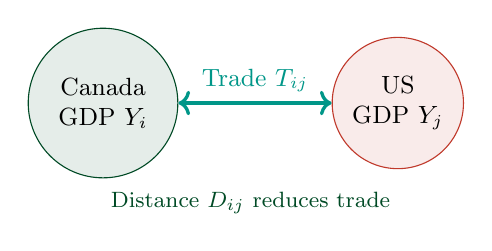
\begin{tikzpicture}[scale=0.78,every node/.style={font=\small}]
  \node[draw=UNBCDark,fill=UNBCDark!10,circle,
        minimum size=1.9cm,align=center] (H) at (0,0)
    {Canada\\GDP $Y_i$};
  \node[draw=AccentRed,fill=AccentRed!10,circle,
        minimum size=1.5cm,align=center] (F) at (4.8,0)
    {US\\GDP $Y_j$};
  \draw[<->,very thick,AccentTeal] (H.east)--(F.west)
    node[midway,above,font=\small,AccentTeal] {Trade $T_{ij}$};
  \node[below=0.3cm,font=\footnotesize,UNBCDark] at (2.4,-0.9)
    {Distance $D_{ij}$ reduces trade};
\end{tikzpicture}
\vspace{0.3em}
\begin{insight}{Canada's Lucky Geography}
\small Canada sits beside the world's largest economy (\$27T GDP) at minimal effective distance. The gravity model predicts enormous Canada–US trade -- and that is exactly what we observe.
\end{insight}
\end{column}
\end{columns}
\end{frame}

%% ─────────────────────────────────────────────────────────────
%% 9. GRAVITY — THE EQUATION
%% ─────────────────────────────────────────────────────────────
\begin{frame}{The Gravity Model -- The Equation}
\begin{columns}[T]
\begin{column}{0.54\textwidth}
\begin{block}{The Gravity Equation}
\[T_{ij} \;=\; A\;\cdot\;\frac{Y_i^{\,\alpha}\;Y_j^{\,\beta}}{D_{ij}^{\,\gamma}} \;\cdot\; \exp\!\bigl(\mathbf{z}_{ij}'\,\delta\bigr)\]
\end{block}
\vspace{0.2em}
\begin{varbox}
\footnotesize
$T_{ij}$: bilateral trade from country $i$ to $j$\\
$Y_i, Y_j$: GDP of exporter and importer\\
$D_{ij}$: bilateral distance (great-circle km)\\
$\mathbf{z}_{ij}$: frictions (language, border, FTA, colonial tie)\\
$A$: scale constant\\
$\alpha,\beta\approx 1$: GDP elasticities\\
$\gamma\approx 0.7$–$1.0$: distance elasticity\\
$\delta$: friction coefficients
\end{varbox}
\end{column}
\begin{column}{0.43\textwidth}
\textbf{Log-linear form (used in OLS):}
\[\ln T_{ij} = c + \alpha\ln Y_i + \beta\ln Y_j - \gamma\ln D_{ij} + \mathbf{z}_{ij}'\delta\]
\vspace{0.2em}
\begin{adjustbox}{max width=\columnwidth}
\begin{tabular}{lc}
\toprule
\textbf{Bilateral feature $z_{ij}$} & \textbf{Effect on $T$}\\
\midrule
Common language    & $+35$–$55\%$\\
Contiguous border  & $+25$–$50\%$\\
FTA membership     & $+40$–$80\%$\\
Colonial relationship & $+20$–$40\%$\\
Currency union     & $+70$–$120\%$\\
\bottomrule
\multicolumn{2}{l}{\tiny Source: Head \& Mayer (2014)}
\end{tabular}
\end{adjustbox}
\end{column}
\end{columns}
\end{frame}

%% ─────────────────────────────────────────────────────────────
%% 10. GRAVITY — READING COEFFICIENTS
%% ─────────────────────────────────────────────────────────────
\begin{frame}{Reading Gravity Coefficients: What Do They Tell Us?}


\textbf{Log-linear gravity:}
\[\ln T = c + \underbrace{\alpha\ln Y_i}_{\text{exporter size}} + \underbrace{\beta\ln Y_j}_{\text{importer size}} \underbrace{-\,\gamma\ln D_{ij}}_{\text{distance}}\]
\textbf{Interpretation:}
\begin{itemize}\small
  \item \textbf{$\alpha=\beta=1$}: 10\% bigger economy $\Rightarrow$ 10\% more trade. Proportional to size.
  \item \textbf{$\gamma=1$}: 10\% farther $\Rightarrow$ 10\% \emph{less} trade. Robust across all samples since 1970.
  \item \textbf{FTA dummy $\delta\approx 0.5$}: $e^{0.5}\approx 1.65$, so FTA raises trade $\approx65\%$ (holding GDP and distance fixed).
\end{itemize}



\end{frame}

%% ─────────────────────────────────────────────────────────────
%% 11. GRAVITY — WORKED EXAMPLE (SETUP)
%% ─────────────────────────────────────────────────────────────
\begin{frame}{Gravity Model -- Worked Example: Setup}
\begin{columns}[T]
\begin{column}{0.50\textwidth}
\begin{worked}
$T_{ij} = A\cdot\dfrac{Y_i\,Y_j}{D_{ij}}$,\quad $A=1$ (\$billion, km).
\end{worked}
\vspace{0.3em}
\textbf{Data:}
\begin{center}
\begin{adjustbox}{max width=0.95\columnwidth}
\begin{tabular}{lcc}
\toprule
Country pair & GDP product & Distance\\
\midrule
A (Canada) -- B (USA) & \$2{,}000B $\times$ \$15{,}000B & 1{,}000 km\\
A (Canada) -- C (Japan) & \$2{,}000B $\times$ \$5{,}000B & 10{,}000 km\\
\bottomrule
\end{tabular}
\end{adjustbox}
\end{center}


\end{column}
\begin{column}{0.47\textwidth}
\textbf{Questions:}
\begin{enumerate}[(a)]\small
  \item Compute $T_{AB}$ and $T_{AC}$.
  \item Find the ratio $T_{AB}/T_{AC}$.
  \item A CPTPP-style agreement \textbf{halves} effective distance to Japan. Compute new $T_{AC}^{\text{FTA}}$.
  \item What does ``effective distance'' capture beyond physical km?
\end{enumerate}
\vspace{0.3em}
\textit{Try it now -- solution on next slide.}
\end{column}
\end{columns}
\end{frame}

%% ─────────────────────────────────────────────────────────────
%% 12. GRAVITY — WORKED EXAMPLE (SOLUTION)
%% ─────────────────────────────────────────────────────────────
\begin{frame}{Gravity Model -- Worked Example: Solution}
\begin{columns}[T]
\begin{column}{0.52\textwidth}
\textbf{(a)} Predicted trade:
\[T_{AB} = \frac{2{,}000\times15{,}000}{1{,}000} = \mathbf{30{,}000}\]
\[T_{AC} = \frac{2{,}000\times5{,}000}{10{,}000} = \mathbf{1{,}000}\]
\textbf{(b)} Ratio: $\;T_{AB}/T_{AC} = \mathbf{30}$\\[0.3em]
Canada trades \textbf{30$\times$ more} with the US than with Japan.\\[0.3em]
\textbf{(c)} CPTPP halves distance to 5{,}000 km:
\[T_{AC}^{\text{FTA}} = \frac{2{,}000\times5{,}000}{5{,}000} = \mathbf{2{,}000}\quad\text{(doubled)}\]
\end{column}
\begin{column}{0.45\textwidth}
\textbf{(d) ``Effective distance'' captures:}
\begin{itemize}\small
  \item \textbf{Tariffs}: $t$\% tariff $\Rightarrow$ higher effective price.
  \item \textbf{Regulatory barriers}: standards, certificates, inspections.
  \item \textbf{Information costs}: unfamiliarity with distant markets.
  \item \textbf{Language/legal}: harder to negotiate and enforce contracts.
\end{itemize}

\end{column}
\end{columns}
\end{frame}



%% ─────────────────────────────────────────────────────────────
%% 14. GRAVITY ANOMALIES
%% ─────────────────────────────────────────────────────────────


%% ═══════════════════════════════════════════════════════════
%%  PART 3 — DISTANCE AND BORDERS
%% ═══════════════════════════════════════════════════════════

%% ─────────────────────────────────────────────────────────────
%% 15. WHY DISTANCE STILL MATTERS
%% ─────────────────────────────────────────────────────────────
\begin{frame}[shrink=7]{Why Distance Still Matters in the Digital Age}
\begin{columns}[T]
\begin{column}{0.53\textwidth}
\begin{alertblock}{Empirical finding}
\small A \textbf{1\% increase in distance} reduces bilateral trade by \textbf{0.7--1.0\%} even controlling for GDP. This effect has \emph{not} declined since 1970.
\end{alertblock}
\vspace{0.2em}
\textbf{Five channels:}
\begin{enumerate}\small
  \item \textbf{Transport costs}: bulk goods (oil, grain, lumber, cars) are expensive to ship far.
  \item \textbf{Time costs}: just-in-time supply chains demand proximity.
  \item \textbf{Information and trust}: close partners are better known.
  \item \textbf{After-sale service}: technical support requires local presence.
  \item \textbf{Regional networks}: USMCA, EU, ASEAN amplify neighbour trade.
\end{enumerate}
\end{column}
\begin{column}{0.44\textwidth}
\begin{canadex}[BC Lumber: Distance vs.\ Demand]
\footnotesize BC exports $\approx$80\% of softwood lumber to the US despite growing Asian demand.\\[0.2em]
\textbf{Why?} Ocean freight to China $\approx4\times$ US corridor cost. Distance costs dominate even in the digital era for \textbf{physical goods}.
\end{canadex}

\end{column}
\end{columns}
\end{frame}

%% ─────────────────────────────────────────────────────────────
%% 16. THE HOME BIAS AND BORDER EFFECT
%% ─────────────────────────────────────────────────────────────
\begin{frame}{The Home Bias Puzzle: Borders Deter More Than We Think}
\begin{columns}[T]
\begin{column}{0.52\textwidth}
\textbf{McCallum (1995) -- a landmark finding:}\\[0.3em]
Comparing Canadian interprovincial trade with Canada–US trade at the same distance, McCallum found that:
\begin{center}
\large\textbf{Canadian provinces traded $\approx20\times$ more with each other than with equally distant US states.}
\end{center}
\vspace{0.2em}
This finding shocked economists -- CUSFTA had \emph{already} eliminated most tariffs. The border effect persisted.\\[0.2em]
Revised estimates (post-NAFTA) put it at $\approx$\textbf{10--12$\times$}, still enormous.
\end{column}
\begin{column}{0.45\textwidth}
\begin{insight}{Interpreting the Border Effect}
\footnotesize The Canada–US border acts as if it adds $\approx$\textbf{75,000 km} of extra distance (Anderson \& van Wincoop 2003).\\[0.3em]
This huge implicit barrier is driven by:
\begin{itemize}\footnotesize
  \item Different regulatory standards and product certifications
  \item Currency exchange costs and USD/CAD uncertainty
  \item Different legal systems 
  \item Customs documentation even under USMCA
  \item Cultural and information differences
\end{itemize}
\end{insight}
\end{column}
\end{columns}
\end{frame}

%% ─────────────────────────────────────────────────────────────
%% 17. FIGURE 2.4 — BC TRADE
%% ─────────────────────────────────────────────────────────────
\begin{frame}{Figure 2-4: BC Trade with Canadian Provinces vs.\ US States}
\begin{columns}[T]
\begin{column}{0.52\textwidth}
\FIG{figures/slide15_img01.png}
\end{column}
\begin{column}{0.45\textwidth}
\textbf{Reading Figure 2-4:}
\begin{itemize}\small
  \item Plots BC trade as \% of GDP against distance from Vancouver.
  \item \textbf{Red (Canadian provinces)}: trade is much higher at every distance.
  \item \textbf{Blue (US states)}: trade is much lower, even for close states.
  \item The \textbf{gap} between the lines = the \emph{border effect}.
\end{itemize}

\end{column}
\end{columns}
\end{frame}

%% ─────────────────────────────────────────────────────────────
%% 18. TABLE 2.1
%% ─────────────────────────────────────────────────────────────
\begin{frame}{Table 2-1: BC Trade as \% of GDP (2009)}
\begin{columns}[T]
\begin{column}{0.52\textwidth}
\begin{center}
\begin{adjustbox}{max width=\columnwidth}
\begin{tabular}{lcc}
\toprule
\textbf{Partner} & \textbf{GDP (C\$B)} & \textbf{BC trade/GDP}\\
\midrule
\multicolumn{3}{l}{\small\textit{Canadian Provinces}}\\
Ontario       & 602 & 6.9\%\\
Alberta       & 323 & 2.6\%\\
Quebec        & 297 & 1.0\%\\
\midrule
\multicolumn{3}{l}{\small\textit{US States}}\\
Washington    & 350 & 0.4\%\\
California    & 1{,}750 & 0.3\%\\
New York      & 1{,}140 & 0.1\%\\
\bottomrule
\multicolumn{3}{l}{\scriptsize Source: Statistics Canada; US Dept.\ of Commerce}
\end{tabular}
\end{adjustbox}
\end{center}
\end{column}
\begin{column}{0.45\textwidth}
\textbf{Key observations:}
\begin{itemize}\small
  \item Ontario (6.9\%) vs.\ Washington State (0.4\%) at similar distances -- a 17$\times$ gap.
  \item California is 3$\times$ larger than Ontario but trades far less with BC.
  \item Border costs explain the entire gap: currency, customs, standards, legal systems.
\end{itemize}
\vspace{0.3em}

\end{column}
\end{columns}
\end{frame}

%% ─────────────────────────────────────────────────────────────
%% 19. BEHIND-THE-BORDER BARRIERS
%% ─────────────────────────────────────────────────────────────
\begin{frame}{Behind-the-Border Barriers: Non-Tariff Costs}

\textbf{Even under zero-tariff CUSMA, barriers remain:}
\begin{enumerate}\small
  \item \textbf{Regulatory differences}: safety, environmental, labelling standards.
  \item \textbf{Rules of origin}: 75\% North American content for autos; creates compliance costs.
  \item \textbf{Currency risk}: CAD/USD fluctuations add contract uncertainty.
  \item \textbf{Legal differences}: contract enforcement
  \item \textbf{``Buy American''}: US government procurement preferences.
\end{enumerate}
\vspace{0.2em}
\textbf{Frontier}: cutting non-tariff barriers matters more than further tariff cuts.


\end{frame}

%% ═══════════════════════════════════════════════════════════
%%  PART 4 — TWO WAVES OF GLOBALISATION
%% ═══════════════════════════════════════════════════════════

%% ─────────────────────────────────────────────────────────────
%% 20. FIRST WAVE
%% ─────────────────────────────────────────────────────────────
\begin{frame}{Two Waves of Globalisation: The First Wave (1870--1913)}

\textbf{What drove the first wave?}
\begin{itemize}
  \item \textbf{Technology}: steamships cut ocean freight costs by 70\%; railways opened continental interiors; telegraph enabled real-time price information.
  \item \textbf{Monetary framework}: classical gold standard fixed exchange rates and enabled large cross-border capital flows.

\end{itemize}
\vspace{0.2em}
\textbf{Result}: World trade/GDP rose from $\approx$5\% (1850) to $\approx$12\% (1913).

\end{frame}

%% ─────────────────────────────────────────────────────────────
%% 21. RETREAT AND SECOND WAVE
%% ─────────────────────────────────────────────────────────────
\begin{frame}{Retreat (1914--1945) and the Second Wave (1945--)}
\begin{columns}[T]
\begin{column}{0.53\textwidth}
\textbf{Interwar collapse:}
\begin{itemize}\small
  \item WWI shattered trade finance and supply chains.
  \item Great Depression $+$ Smoot-Hawley (1930): US tariff $\approx$45\%.
  \item Retaliatory tariffs worldwide: world trade \textbf{fell 66\%} in 1929--33.
\end{itemize}
\vspace{0.2em}
\textbf{Second wave (1945--):}
\begin{itemize}\small
  \item GATT (1947); Bretton Woods; containerisation (1956).
  \item Trade/GDP exceeded pre-WWI peak by 1970.
  \item WTO (1995); China WTO (2001); GVC explosion.
  \item Post-2008 slowdown; post-2020 fragmentation.
\end{itemize}
\end{column}
\begin{column}{0.44\textwidth}
\begin{insight}{The Political Lesson}
\footnotesize Globalisation requires \emph{both} technology \emph{and} political commitment.\\[0.3em]
Smoot-Hawley reversed decades of liberalisation in two years.\\[0.3em]
GATT/WTO is the institutional safeguard -- but faces strain: US-China tech war, WTO appellate body crisis (2019).
\end{insight}
\end{column}
\end{columns}
\end{frame}

%% ─────────────────────────────────────────────────────────────
%% 22. FIGURE 2.5 — WORLD TRADE OVER TIME
%% ─────────────────────────────────────────────────────────────
\begin{frame}[shrink=5]{Figure 2-5: The Rise, Fall, and Rise of World Trade}
\begin{columns}[T]
\begin{column}{0.54\textwidth}
\FIGS[0.96]{figures/slide20_img01.png}
\end{column}
\begin{column}{0.43\textwidth}
\textbf{Reading Figure 2-5:}
\begin{itemize}\small
  \item \textbf{First peak} $\approx$1913: first globalisation wave.
  \item \textbf{Deep trough} 1914--45: wars, Depression, Smoot-Hawley.
  \item \textbf{Recovery} 1950s--70s: GATT, containerisation.
  \item \textbf{New peak} 1990s--2008: WTO, China, GVCs.
  \item \textbf{Post-2008}: trade grew slower than GDP.
\end{itemize}
\vspace{0.2em}
\begin{canadex}
\footnotesize Canada's export/GDP closely mirrors the world. 2000s boom: NAFTA $+$ China commodity demand.
\end{canadex}
\end{column}
\end{columns}
\end{frame}

%% ─────────────────────────────────────────────────────────────
%% 23. POST-2020 FRAGMENTATION
%% ─────────────────────────────────────────────────────────────
\begin{frame}{Post-2020: The Fragmentation of Global Trade}
\begin{columns}[T]
\begin{column}{0.54\textwidth}
\textbf{New forces reshaping global trade since 2020:}
\begin{itemize}
  \item \textbf{COVID-19}: supply chain disruptions revealed concentration risks (semiconductors, PPE, pharmaceuticals).
  \item \textbf{US-China tech war}: export controls on chips, AI, telecom.
  \item \textbf{Russia-Ukraine war}: energy and food commodity markets disrupted.
  \item \textbf{``Friend-shoring''}: shifting supply chains to geopolitically aligned partners.
  \item \textbf{Industrial policy resurgence}: US Inflation Reduction Act, EU Green Deal — subsidies for domestic production.
\end{itemize}
\end{column}
\begin{column}{0.43\textwidth}
\begin{canadex}[Canada's Opportunity and Risk]
\footnotesize \textbf{Opportunity}: As a trusted US ally, Canada benefits from friend-shoring. EV battery plants (Volkswagen, Stellantis in Ontario) are a direct result.\\[0.3em]
\textbf{Risk}: If global GVCs fragment, Canada's export diversity could fall further toward US dependence.\\[0.3em]
Canadian trade policy under fragmentation must balance \textbf{CUSMA integration} with \textbf{CPTPP and CETA diversification}.
\end{canadex}
\end{column}
\end{columns}
\end{frame}

%% ═══════════════════════════════════════════════════════════
%%  PART 5 — COMPOSITION AND GVCs
%% ═══════════════════════════════════════════════════════════

%% ─────────────────────────────────────────────────────────────
%% 24. COMPOSITION OVERVIEW
%% ─────────────────────────────────────────────────────────────
\begin{frame}{What Do Countries Trade? Composition of World Trade}
\begin{columns}[T]
\begin{column}{0.52\textwidth}
\FIG{figures/slide22_img01.png}
\end{column}
\begin{column}{0.45\textwidth}
\textbf{World merchandise trade (2017):}
\begin{itemize}\small
  \item \textbf{Manufactures $\approx$68\%}: machinery, cars, electronics, chemicals.
  \item \textbf{Fuels/mining $\approx$15\%}: oil, gas, coal, metals.
  \item \textbf{Agriculture $\approx$10\%}: wheat, soybeans, coffee, fish.
\end{itemize}
\vspace{0.2em}
\begin{canadex}[Canada's Unusual Trade Basket]
\footnotesize Canada exports \emph{all three} categories: oil (energy), cars/aircraft (manufacturing), wheat/canola/potash (agriculture).\\[0.2em]
This dual structure makes Canada sensitive to both commodity-price shocks \emph{and} manufacturing-demand shocks -- unusual among G7 peers.
\end{canadex}
\end{column}
\end{columns}
\end{frame}

%% ─────────────────────────────────────────────────────────────
%% 25. TABLE 2.2 — MANUFACTURING SHIFT
%% ─────────────────────────────────────────────────────────────
\begin{frame}{Table 2-2: The Rise of Manufacturing Trade}
\begin{columns}[T]
\begin{column}{0.50\textwidth}
\begin{center}
\begin{adjustbox}{max width=\columnwidth}
\begin{tabular}{lcccc}
\toprule
\textbf{Country} & \textbf{1910 exp.} & \textbf{1910 imp.} & \textbf{2002 exp.} & \textbf{2002 imp.}\\
\midrule
UK & 75\% & 24\% & 82\% & 79\%\\
US & 47\% & 40\% & 84\% & 77\%\\
\bottomrule
\multicolumn{5}{l}{\scriptsize\textit{Source: Kuznets (1967); WTO}}
\end{tabular}
\end{adjustbox}
\end{center}
\vspace{0.3em}
\textbf{The shift:}
\begin{itemize}\small
  \item \textbf{1910}: UK exported manufactures, imported primary goods. \emph{Inter-industry} trade.
  \item \textbf{2002}: Both UK exports \emph{and} imports are manufactures. This is \emph{intra-industry} trade.
\end{itemize}
\end{column}
\begin{column}{0.47\textwidth}
\begin{varbox}
\footnotesize\textbf{Inter-industry vs.\ intra-industry:}\\[0.25em]
\textbf{Inter-industry}: Canada exports wheat, imports electronics. Explained by comparative advantage (Ch.~3--5).\\[0.3em]
\textbf{Intra-industry}: Canada both exports and imports cars. Explained by economies of scale (Ch.~7).
\end{varbox}
\vspace{0.3em}
\begin{insight}{Macro Connection}
\footnotesize Manufacturing demand is more cyclical than agriculture. Countries specialised in manufactures have more volatile trade balances -- relevant for Canadian monetary policy.
\end{insight}
\end{column}
\end{columns}
\end{frame}

%% ─────────────────────────────────────────────────────────────
%% 26. DEVELOPING COUNTRY TRANSFORMATION
%% ─────────────────────────────────────────────────────────────
\begin{frame}[shrink=6]{The Transformation of Developing Country Exports}
\begin{columns}[T]
\begin{column}{0.52\textwidth}
\FIG{figures/slide26_img01.jpg}
\end{column}
\begin{column}{0.45\textwidth}
\textbf{A remarkable structural shift:}
\begin{itemize}\small
  \item \textbf{1960}: $\approx$58\% of developing exports were primary commodities.
  \item \textbf{2001}: $\approx$65\% were manufactures.
  \item \textbf{China}: $>$90\% manufactures; moving toward AI and semiconductors.
\end{itemize}
\vspace{0.2em}
\begin{adjustbox}{max width=\columnwidth}
\begin{tabular}{lcc}
\toprule
Country & Mfg.\% 1960 & Mfg.\% 2019\\
\midrule
China       & 10 & 93\\
South Korea & 20 & 89\\
Bangladesh  &  5 & 90\\
\bottomrule
\end{tabular}
\end{adjustbox}

\end{column}
\end{columns}
\end{frame}

%% ─────────────────────────────────────────────────────────────
%% 27. GLOBAL VALUE CHAINS
%% ─────────────────────────────────────────────────────────────
\begin{frame}{Global Value Chains: ``Made in the World''}
\begin{columns}[T]
\begin{column}{0.53\textwidth}
\textbf{Modern production is internationally fragmented:}
\begin{itemize}\small
  \item Design, components, assembly, and retail done in \emph{different countries}.
  \item A \$500 smartphone may cross \textbf{6 borders} before reaching a consumer.
  \item Gross exports \emph{overstate} domestic content: Chinese re-exports of Malaysian components count as Chinese exports.
\end{itemize}
\vspace{0.2em}
\begin{insight}{Policy Issue}
\footnotesize Tariffs on intermediate inputs hurt domestic assemblers. US 2018 steel tariffs raised costs for US automakers -- including USMCA Canadian plants.
\end{insight}
\end{column}
\begin{column}{0.44\textwidth}
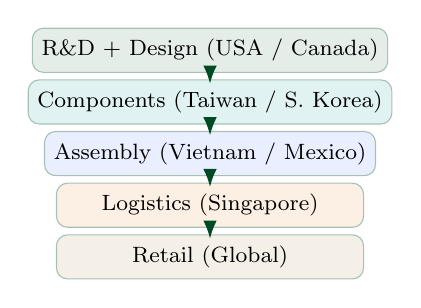
\begin{tikzpicture}[scale=0.82,every node/.style={font=\footnotesize}]
  \foreach \y/\fc/\t in {
      3.6/UNBCDark!10/{R\&D + Design (USA / Canada)},
      2.8/AccentTeal!12/{Components (Taiwan / S.\ Korea)},
      2.0/AccentBlue!10/{Assembly (Vietnam / Mexico)},
      1.2/AccentOrange!12/{Logistics (Singapore)},
      0.4/UNBCGold!15/{Retail (Global)}}{
    \node[draw=UNBCDark!35,fill=\fc,rounded corners,
          minimum width=3.9cm,minimum height=0.56cm,align=center]
      at (0,\y) {\t};
  }
  \foreach \ya/\yb in {3.32/3.08,2.52/2.28,1.72/1.48,0.92/0.68}
    \draw[-{Latex},UNBCDark,thick] (0,\ya)--(0,\yb);
\end{tikzpicture}
\end{column}
\end{columns}
\end{frame}

%% ─────────────────────────────────────────────────────────────
%% 28. SERVICE OFFSHORING
%% ─────────────────────────────────────────────────────────────
\begin{frame}{Service Trade: The New Frontier}
\begin{columns}[T]
\begin{column}{0.52\textwidth}
\FIG{figures/slide29_img01.jpg}
\end{column}
\begin{column}{0.45\textwidth}
\textbf{Services trade is fast-growing:}
\begin{itemize}\small
  \item World services trade $\approx$\$6T (2019): fastest-growing category.
  \item \textbf{Tradable}: IT, finance, engineering, education, radiology.
  \item \textbf{Non-tradable}: haircuts, local retail, most healthcare.
\end{itemize}
\vspace{0.2em}
\begin{canadex}
\footnotesize Canada: \textbf{net importer} of IT services (US/India), \textbf{net exporter} of financial services, engineering consulting, education.\\[0.2em]
$\approx$850{,}000 international students/year -- a large ``invisible'' Canadian export.
\end{canadex}
\end{column}
\end{columns}
\end{frame}

%% ═══════════════════════════════════════════════════════════
%%  PART 6 — CANADIAN MACRO CONNECTIONS
%% ═══════════════════════════════════════════════════════════

%% ─────────────────────────────────────────────────────────────
%% 29. WHEN US SNEEZES
%% ─────────────────────────────────────────────────────────────
\begin{frame}{When the US Sneezes, Canada Catches a Cold}
\begin{columns}[T]
\begin{column}{0.54\textwidth}
\textbf{Trade transmission mechanism:}
\begin{enumerate}\small
  \item \textbf{US recession}: US aggregate demand falls.
  \item \textbf{Canadian exports fall}: $\Delta X < 0 \Rightarrow \Delta\text{NX} < 0$.
  \item \textbf{Canadian GDP falls}: $\Delta Y < 0$.
  \item \textbf{Unemployment rises}: Ontario auto, BC forestry, Alberta oil.
  \item \textbf{Bank of Canada responds}: cuts overnight rate.
  \item \textbf{CAD depreciates}: partial export offset.
\end{enumerate}
\vspace{0.2em}
\begin{insight}{2008--09 Case}
\footnotesize Canada entered recession months after the US financial crisis despite no domestic housing bubble. BoC cut rates from 4.5\% to 0.25\% within one year.
\end{insight}
\end{column}
\begin{column}{0.43\textwidth}
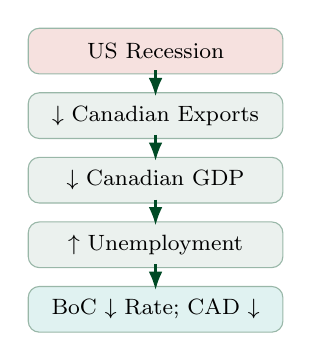
\begin{tikzpicture}[scale=0.82,every node/.style={font=\footnotesize}]
  \foreach \y/\fc/\t in {
      4.5/AccentRed!15/{US Recession},
      3.5/UNBCDark!8/{$\downarrow$ Canadian Exports},
      2.5/UNBCDark!8/{$\downarrow$ Canadian GDP},
      1.5/UNBCDark!8/{$\uparrow$ Unemployment},
      0.5/AccentTeal!12/{BoC $\downarrow$ Rate; CAD $\downarrow$}}{
    \node[draw=UNBCDark!40,fill=\fc,rounded corners,
          text width=3.0cm,minimum height=0.58cm,align=center]
      at (0,\y) {\t};
  }
  \foreach \ya/\yb in {4.2/3.8,3.2/2.8,2.2/1.8,1.2/0.8}
    \draw[-{Latex},UNBCDark,thick] (0,\ya)--(0,\yb);
\end{tikzpicture}
\end{column}
\end{columns}
\end{frame}

%% ─────────────────────────────────────────────────────────────
%% 30. COMMODITY PRICES AND TERMS OF TRADE
%% ─────────────────────────────────────────────────────────────
\begin{frame}{Commodity Prices and Canada's Terms of Trade}

\textbf{Terms of trade} (ToT) $= P_{\text{exports}}/P_{\text{imports}}$.\\[0.3em]
For Canada (resource exporter), oil prices drive ToT:
\begin{itemize}\small
  \item Oil $\uparrow \Rightarrow$ ToT improve $\Rightarrow$ real income rises above real GDP.
  \item Oil $\downarrow \Rightarrow$ ToT worsen $\Rightarrow$ Alberta/Saskatchewan recession.
\end{itemize}
\vspace{0.3em}
\begin{adjustbox}{max width=\columnwidth}
\begin{tabular}{lcc}
\toprule
Period & Oil price & Canadian effect\\
\midrule
2002--14 & \$25$\to$\$110 & ToT $\uparrow$ 40\%; boom\\
2014--16 & \$110$\to$\$45 & Alberta recession; CAD \$0.68\\
2021--22 & \$45$\to$\$110 & ToT recovered; CAD strengthened\\
\bottomrule
\end{tabular}
\end{adjustbox}

\end{frame}

%% ─────────────────────────────────────────────────────────────
%% 31. DUTCH DISEASE
%% ─────────────────────────────────────────────────────────────
\begin{frame}[shrink=7]{Dutch Disease: When Resource Wealth Hurts Manufacturing}
\begin{columns}[T]
\begin{column}{0.53\textwidth}
\textbf{The Dutch Disease mechanism:}
\begin{enumerate}\small
  \item Commodity boom raises Canada's export revenues.
  \item Increased foreign demand for CAD pushes CAD higher.
  \item Higher CAD makes Canadian manufactured exports more expensive for foreign buyers.
  \item Manufacturing exports fall; factory closures and job losses in Ontario/Quebec.
  \item Resource sector booms while manufacturing sector ``hollows out.''
\end{enumerate}
\vspace{0.2em}
\textbf{Historical case:}\\
2007--2012: CAD reached parity with USD. Ontario auto and forestry exports fell sharply. ``Dutch Disease'' debate dominated Canadian economic policy discussion.
\end{column}
\begin{column}{0.44\textwidth}
\begin{insight}{Named After the Netherlands}
\footnotesize In the 1960s, the Netherlands discovered North Sea natural gas. Gas export revenues pushed up the Dutch guilder.\\[0.2em]
Dutch manufactured exports became uncompetitive. Manufacturing employment fell sharply -- even though the country became richer overall.\\[0.2em]
The \textbf{distributional effect}: resource-sector workers gain; manufacturing-sector workers lose -- connecting to the Specific Factors Model (Ch.~4).
\end{insight}
\end{column}
\end{columns}
\end{frame}

%% ─────────────────────────────────────────────────────────────
%% 32. EXCHANGE RATE PREVIEW
%% ─────────────────────────────────────────────────────────────
\begin{frame}{Exchange Rates and Trade Competitiveness: A Preview}
\begin{columns}[T]
\begin{column}{0.54\textwidth}
\textbf{Trade and exchange rates are deeply linked:}
\begin{itemize}\small
  \item Let $e$ = USD per 1 CAD ($\uparrow e$ = CAD appreciates).
  \item Price of Canadian export in USD: $\;P_{\text{USD}} = e \cdot P_{\text{CAD}}$.
  \item \textbf{CAD appreciates} ($e\uparrow$): Canadian exports more expensive $\Rightarrow$ volumes fall.
  \item \textbf{CAD depreciates} ($e\downarrow$): Canadian exports cheaper $\Rightarrow$ volumes rise.
\end{itemize}
\vspace{0.2em}
\textbf{2007--2012}: CAD at parity with USD. Canadian manufacturers lost competitiveness; BC lumber exports fell sharply. The ``Dutch Disease'' debate.
\end{column}
\begin{column}{0.43\textwidth}
\begin{varbox}
\footnotesize\textbf{Real exchange rate:}\\[0.2em]
$q = \dfrac{e \cdot P^*}{P}$\\[0.2em]
$P^*$ = US price level, $P$ = Canadian\\[0.2em]
$q \uparrow$ = Canada more competitive\\
$q \downarrow$ = Canada less competitive\\[0.3em]
Full treatment in macroeconomics. Here: the direction of the effect matters for understanding trade volume.
\end{varbox}
\end{column}
\end{columns}
\end{frame}

%% ─────────────────────────────────────────────────────────────
%% 33. TRADE DIVERSIFICATION DEBATE
%% ─────────────────────────────────────────────────────────────
\begin{frame}{Should Canada Diversify Away from the US?}
\begin{columns}[T]
\begin{column}{0.54\textwidth}
\textbf{The case for diversification:}
\begin{itemize}\small
  \item 75\% US dependence creates macroeconomic vulnerability.
  \item US political risk: tariff threats, CUSMA renegotiations.
  \item CPTPP (2018) and CETA (2017) open new corridors.
\end{itemize}
\vspace{0.2em}
\textbf{The gravity model's answer:}
\begin{itemize}\small
  \item US proximity plus USMCA will remain dominant.
  \item Effective distance to Japan ($\approx$10{,}000 km) vs.\ the US ($\approx$1{,}000 km) means gravity strongly favours the US.
  \item Diversification is possible but the model predicts limited impact.
\end{itemize}
\end{column}
\begin{column}{0.43\textwidth}
\begin{discuss}
\footnotesize
\begin{enumerate}\footnotesize
  \item Can CPTPP realistically cut Canada's US export share below 65\%?
  \item If the US imposed a 10\% tariff on Canadian goods, what would happen to Canadian GDP, employment, and the exchange rate?
  \item Is trade diversification genuine policy or political signalling?
\end{enumerate}
\end{discuss}
\end{column}
\end{columns}
\end{frame}

%% ═══════════════════════════════════════════════════════════
%%  PART 7 — SYNTHESIS AND WRAP-UP
%% ═══════════════════════════════════════════════════════════

%% ─────────────────────────────────────────────────────────────
%% 34. FIVE KEY FACTS
%% ─────────────────────────────────────────────────────────────
\begin{frame}{Five Key Facts About World Trade}

\begin{enumerate}\small
  \item \textbf{Gravity rules}: trade rises with GDP and falls with distance. Borders remain huge barriers even under FTAs.
  \item \textbf{Globalisation is political}: it reversed dramatically 1914--45. Technology enables; institutions sustain.
  \item \textbf{Manufactures dominate}; services trade grows fastest. Developing countries shifted from commodities to manufactures.
  \item \textbf{GVCs define modern trade}: production is internationally fragmented; gross exports overstate domestic content.
  \item \textbf{Trade drives Canadian macro}: exports $\approx$32\% of GDP; US the dominant partner; commodity prices and US cycles transmit through trade.
\end{enumerate}

\end{frame}

%% ─────────────────────────────────────────────────────────────
%% 35. COURSE ROADMAP
%% ─────────────────────────────────────────────────────────────
\begin{frame}{Course Roadmap: Where We Go From Here}
\begin{center}
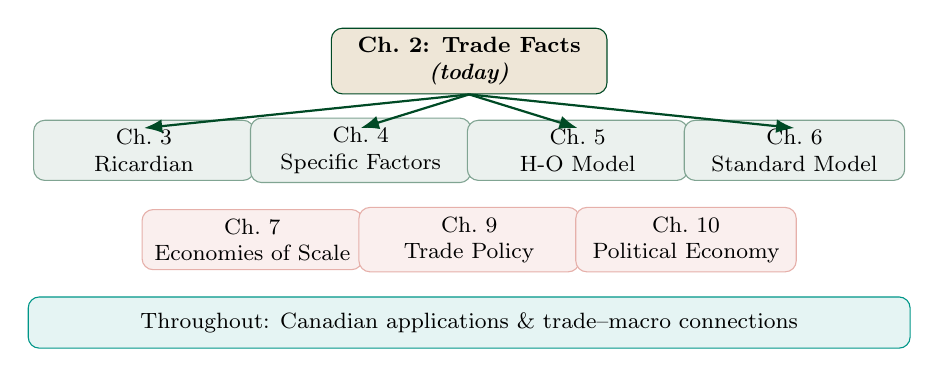
\begin{tikzpicture}[scale=0.81,every node/.style={font=\footnotesize}]
  %% Chapter 2 (today)
  \node[draw=UNBCDark,fill=UNBCGold!25,rounded corners,
        minimum width=3.5cm,minimum height=0.75cm,
        align=center,font=\footnotesize\bfseries] (ch2) at (0,4.3)
    {Ch.~2: Trade Facts \\ \textit{(today)}};
  %% Micro theory row
  \foreach \x/\t in {
      -5.1/{Ch.~3\\Ricardian},
      -1.7/{Ch.~4\\Specific Factors},
       1.7/{Ch.~5\\H-O Model},
       5.1/{Ch.~6\\Standard Model}}{
    \node[draw=UNBCDark!50,fill=UNBCDark!8,rounded corners,
          minimum width=2.8cm,minimum height=0.7cm,align=center]
      at (\x,2.9) {\t};
    \draw[-{Latex},UNBCDark,thick] (ch2.south)--(\x,3.25);
  }
  %% Policy row
  \foreach \x/\fc/\t in {
      -3.4/AccentRed!8/{Ch.~7\\Economies of Scale},
       0.0/AccentRed!8/{Ch.~9\\Trade Policy},
       3.4/AccentRed!8/{Ch.~10\\Political Economy}}{
    \node[draw=AccentRed!40,fill=\fc,rounded corners,
          minimum width=2.8cm,minimum height=0.7cm,align=center]
      at (\x,1.5) {\t};
  }
  %% Thread
  \node[draw=AccentTeal,fill=AccentTeal!10,rounded corners,
        minimum width=11.2cm,minimum height=0.65cm,align=center]
    at (0,0.2) {Throughout: Canadian applications \& trade--macro connections};
\end{tikzpicture}
\end{center}
\end{frame}

%% ─────────────────────────────────────────────────────────────
%% 36. DISCUSSION QUESTIONS + FURTHER READING
%% ─────────────────────────────────────────────────────────────
\begin{frame}[shrink=5]{Discussion Questions and Further Reading}
\begin{columns}[T]
\begin{column}{0.52\textwidth}
\textbf{For next class:}
\begin{enumerate}\small
  \item Gravity predicts Canada will always trade mainly with the US. Does this mean CPTPP is a waste? Defend your view.
  \item $\gamma\approx1$ has not fallen despite the internet. Does this mean digital trade is \emph{not} growing? Explain the difference.
  \item If Canada imposed a 10\% tariff on US goods (breaking CUSMA), what happens to Canadian GDP, inflation, and the exchange rate?
\end{enumerate}
\vspace{0.3em}
\textbf{Key papers:}
\begin{itemize}\footnotesize
  \item McCallum (1995), ``National Borders Matter,'' \textit{AER}.
  \item Anderson \& van Wincoop (2003), ``Gravity with Gravitas,'' \textit{AER}.
  \item Head \& Mayer (2014), ``Gravity Equations: Workhorse, Toolkit, Cookbook.''
\end{itemize}
\end{column}
\begin{column}{0.45\textwidth}
\begin{block}{Key Takeaways}
\begin{itemize}\footnotesize
  \item Gravity: GDP $\uparrow \Rightarrow$ trade $\uparrow$; distance $\uparrow \Rightarrow$ trade $\downarrow$.
  \item Borders: huge implicit barriers even under FTAs.
  \item Globalisation: comes in waves; institutions sustain it.
  \item Composition: shifting toward services and GVCs.
  \item For Canada: trade \emph{is} macroeconomic policy.
\end{itemize}
\end{block}
\vspace{0.3em}
\begin{block}{Next Lecture}
\footnotesize Ch.~3 -- Ricardian Model: Why do countries trade? What determines export patterns?
\end{block}
\end{column}
\end{columns}
\end{frame}

\end{document}
